\documentclass[12pt,a4paper]{article}
\usepackage[utf8]{inputenc}
\usepackage{amsmath}
\usepackage{amsfonts}
\usepackage{amssymb}
\usepackage{graphicx}
\usepackage[left=2cm,right=2cm,top=2cm,bottom=2cm]{geometry}
\author{leonardo}
\title{amplificacion on conexion darlignton}
\begin{document}
\section{marco teorico }
\begin{flushleft}
 El transistor T1 entrega la corriente que sale por su emisor a la base del transistor T2. La ecuación de ganancia de un transistor típico es: IE= β x IB (Corriente de colector es igual a beta por la corriente de base). Entonces analizando el gráfico:

Ecuación del primer transistor es: IE1 = β1 x IB1 (1).
Ecuación del segundo transistor es: IE2 = β2 x IB2 (2).
Observando el gráfico se ve que la corriente de emisor del transistor (T1) es la misma que la corriente de base del transistor T2. Entonces IE1 = IB2 (3). Entonces utilizando la ecuación (2) y la ecuación (3) se obtiene: IE2 = β2 x IB2 = β2 x IE1

Reemplazando en la ecuación anterior el valor de IE1 (ver ecuación (1) ) se obtiene la ecuación final de ganancia del transistor Darlington. IE2 = β2 x β1 x IB1. Como se puede ver, este transistor tiene una ganancia de corriente mucho mayor que la de un transistor común, pues aprovecha la ganancia de los dos transistores. (las ganancias se multiplican).
\end{flushleft}
\begin{flushleft}
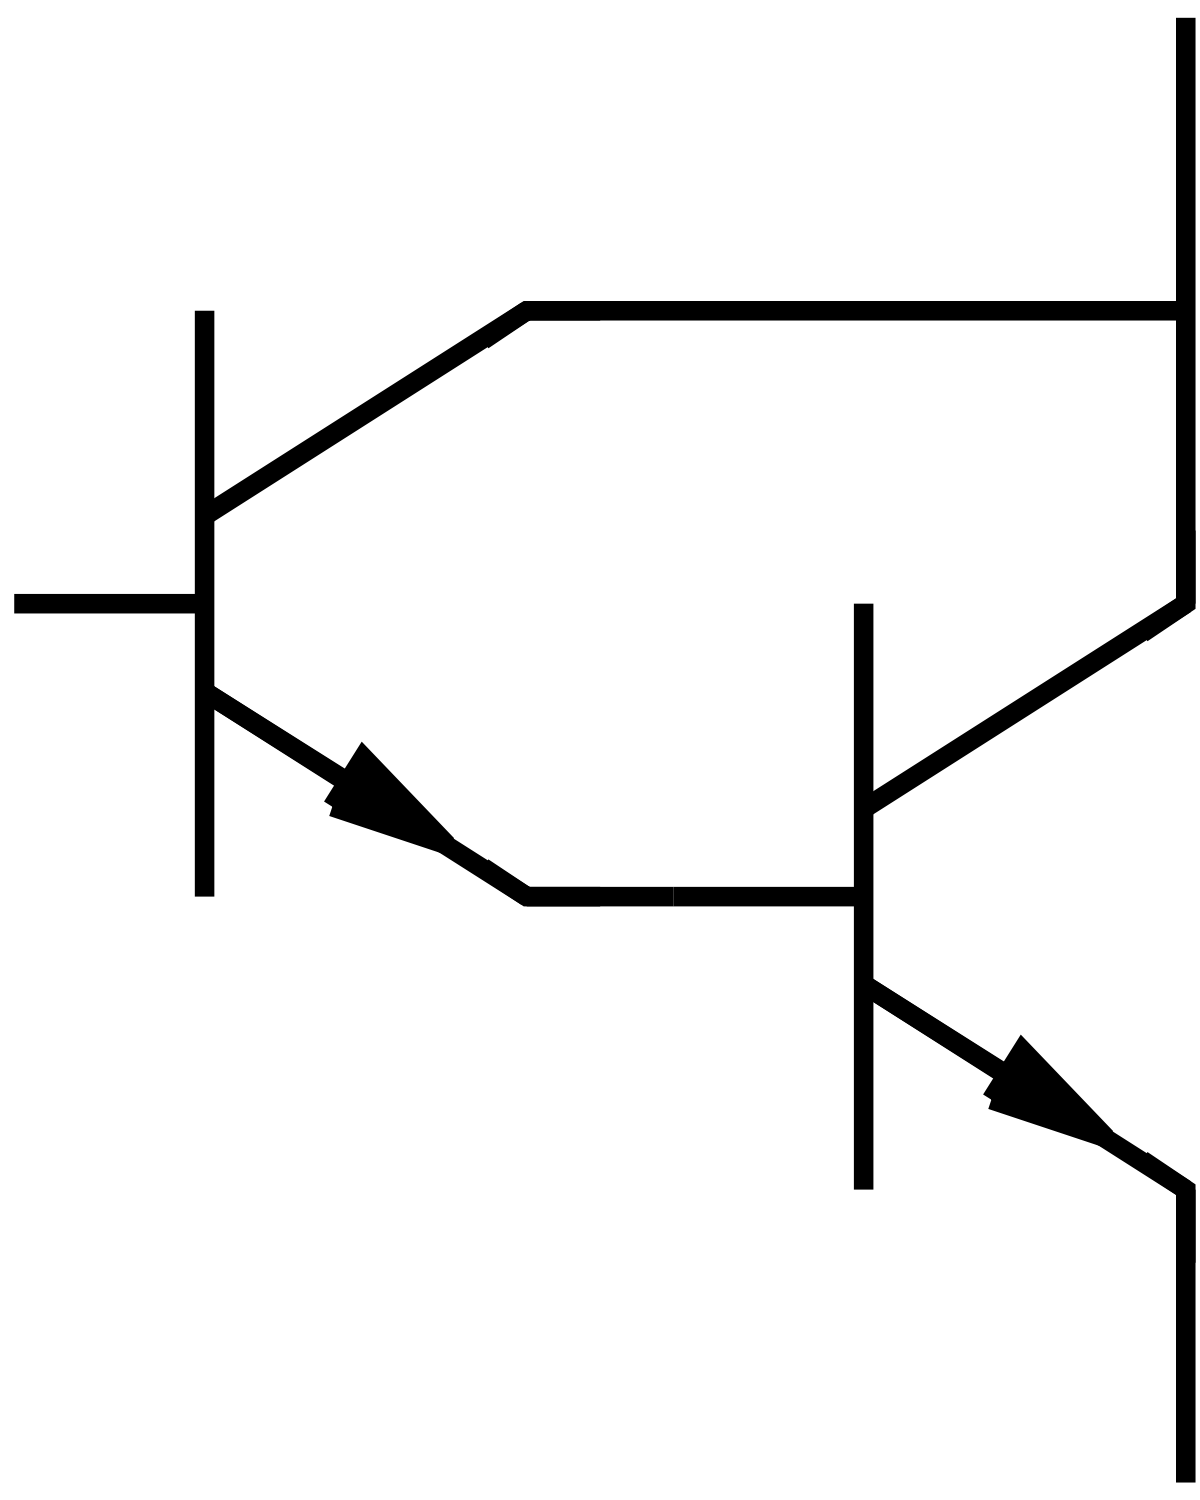
\includegraphics[width=7cm]{1.png} 
\end{flushleft}
\begin{flushleft}
\section{Materiales}
\end{flushleft}
\begin{flushleft}
1.-rotoboard 
\end{flushleft}
\begin{flushleft}
2.- transistores
\end{flushleft}
\begin{flushleft}
3.-dupons
\end{flushleft}
\begin{flushleft}
4.-fotoresistencias
\end{flushleft}
\begin{flushleft}
5.-relevadores
\end{flushleft}



\section{proccedimiento}
\begin{flushleft}
En la practica hicimos la conexion darlington la cual veiamos como se activaban el relevador al orpimir un push botton. tambien hicimos una conexion la cual veiamos como se conectaba una fotoresistencia al activarse se enciende el relevador.

\end{flushleft}
\section{Conclusion}
\begin{flushleft}
 en esta practica entendemos como funciona la fotoresistencia ademas vemos que activa el rlevador la cual es de 5v. En la segunda parte vemos como con la conexion de darligton podemos activar el relevador 

\end{flushleft}
\end{document}